%!TEX root = thesis.tex

\chapter{Simulator documentation}

This chapter provides a documentation for the simulation solution that was developed during this project. 
Some of the steps, described within this documentation require basic knowledge about using the V-Rep scene editor.


\section{Installation and startup}

The simulator plugin code as well as the scene and model files is located in the \texttt{iis\_simulation} package which is part of the \texttt{iis\_robot\_sw} repository. The plugin code was written in C++ and needs to be compiled, using the catkin build system which is part of the ROS distribution. Detailed information about how to install and build the source code can be found in the top-level README file within the repository. The compilation process generates a library file, named \path{libv_RepExtSimulatorPlugin.so}. To be able to work, that library file needs to be copied into the working directory of the V-Rep installation. This happens automatically when using the top-level makefile of the \texttt{iis\_robot\_sw} repository. The plugin library is automatically detected and loaded during V-Rep startup. But as it's functionality depends on ROS it will be unloaded immediately if no running roscore can be detected. The status of recognized plugins can be seen on the console output. \\

The package contains the reference scene file, called \path{scenes/model_assembled.ttt} which can be started, using the \path{robot_scene.launch} file. The command
\begin{verbatim}
roslaunch iis_simulation robot_scene.launch scene:=MY_CUSTOM_SCENE.ttt
\end{verbatim}
starts an instance of V-Rep, loads the scene file provided with the (optional) \texttt{scene} parameter and starts the simulation. If no scene file is provided, the default scene is loaded which is the provided reference scene. Scene files have to reside in the \path{scenes} folder within the package, otherwise the launch file is not able to locate them.

\section{Modifying the simulation scene}

The reference scene contains a fully functional replication of the IIS lab robot setup, composed from two arms, two grippers and a Kinect camera. It is recommended to start with the setup within this file to create alternative scenes and store modified versions in different files. The base of each arm is marked by a dummy element at root level of the scene hierarchy, i.e. \path{dummy_frame_left_arm} and \path{dummy_frame_right_arm}. Modifying the mounting of the arms is done by changing the alignment of those dummy elements. Currently they are placed relative to the origin of the world reference frame. Parts of the scene can safely be deleted without breaking the functionality. To delete a gripper, it's base element has to be located in the scene hierarchy. This is done by expanding the model tree of the corresponding arm until the gripper base  can be selected and removed. Each other part contained within the scene can be removed or rearranged in the same way (table, torso, Kinect camera).\\

The dummy element called \path{ref_frame_origin} states the origin of the reference frame used by the arm controllers and is indicated by a slightly green shimmering sphere near the top left corner of the table. Cartesian positions received from and sent to the arms are interpreted relative to that reference frame. The origin can be changed easily by just modifying the position and orientation of that dummy
element. If it is removed than all positions are interpreted to be relative to the absolute world reference frame (which is currently at the same location).

\section{Modifying custom developer data tags}

Important parts within the scene hierarchy have to be tagged with custom developer data tags, as explained in Section\ref{sec:comp_id}.
\begin{figure}[h]
	\centering
  	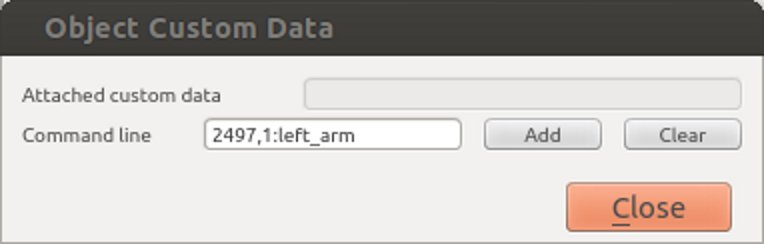
\includegraphics[width=0.7\textwidth]{images/dlg_cust_data.jpg}
	\caption{Edit custom developer data dialog}
	\label{fig:change_dev_data}
\end{figure} 

To edit those data segments, the corresponding scene object needs to be selected in the scene hierarchy. After clicking the option \emph{View/edit custom data} within the \texttt{common} section of the \emph{Scene Object Properties} dialog, a new dialog box appears that allows to attach and remove custom data segments. Existing segment have to be removed prior to attaching a new value. This is done by entering the header ID (2497) into the text box and clicking the \texttt{clear} button. That causes all data segments, identified by the given header ID to be deleted on the selected scene object. After that, the new data segment can be attached by entering the proper values into the text box and clicking the \texttt{add} button. The values, entered in the dialog, shown in Figure\ref{fig:change_dev_data} identify a scene object to be the model base of a \emph{LWRArmComponent} with name \path{left_arm}.

\section{ROS interface}

The ROS interface for the simulated robot components is composed from a set of inbound and outbound ROS topics, that can be used to send commands or to retrieve state data. The used topic names follow the IIS lab internal naming conventions. Each topic name has the structure
\begin{verbatim}
[namespace]/[component name]/[control type]/[name]
\end{verbatim}
The namespace is necessary to distinguish between the topics of simulator and real robot. All simulator related topics reside in the \path{simulation} namespace. The component name identifies a specific instance within that namespace, e.g. \texttt{left\_arm} or \texttt{right\_sdh}. This is useful as often more than one instance of the same robot component is used but all of them are utilizing the same topic names. The control type groups sets of topics into different categories. Possible values are \texttt{joint\_control}, \texttt{cartesian\_control}, \texttt{sensoring} and \texttt{settings}. Finally, the chosen name is used to identify the specific topic within the category. The topic \path{/simulation/left_arm/joint_control/move} states the topic named \path{move} in category \path{joint_control} for a simulated component, named \path{left_arm}. \\

The topics are provided by the registered \emph{ComponentControllers} and are dynamically composed, based on the component name. The overall namespace is declared within the \path{initialize()} method of the \emph{ROSServer} class. The component name has to be provided as value segment of the custom developer data tag that identifies the model base of a specific component within the scene. The control type and name segments of the topics are defined within the \path{initialize()} methods of the concrete controller instances. Some of the provided topics are only fake implementations as the corresponding functionality cannot be implemented on the simulator. Therefore they are just added for consistency reasons, but only fake data is published. These include all temperature and impedance related topics. When messages are sent to one of those fake topics, a corresponding warning will be displayed on the console.

\subsection{Arm control topics}

The topics, provided by the \emph{LWRArmController} follow the specification of the \emph{KUKIE} control interface that gets utilized on the real robot arms in the IIS lab. A complete list of the topics, available on the simulator can be found in Table\ref{fig:arm_topics}. Controller related errors are published to the \path{sensoring/error} topic but they are displayed on the console output of the simulator as well. Joint names, used by the \path{joint_control/get_state} topic are defined in the value segments of the custom developer data tags, attached to the arm joints.

\begin{table}[ht]
\small
\begin{tabularx}{\textwidth}{|X|l|c|} \hline
\textbf{Topic} & \textbf{Message type} & \textbf{Direction} \\ \hline

\path{cartesian_control/get_impedance} & \path{iis_kukie/CartesianImpedance} & outbound  \\
\path{cartesian_control/get_pose} & \path{geometry_msgs/Pose} & outbound  \\
\path{cartesian_control/move} & \path{geometry_msgs/Pose} & inbound  \\
\path{cartesian_control/set_impedance} & \path{iis_kukie/CartesianImpedance} & inbound  \\
\path{cartesian_control/set_velocity_limit} & \path{std_msgs/Float32} & inbound  \\

\path{joint_control/get_impedance} & \path{iis_kukie/FriJointImpedance} & outbound  \\
\path{joint_control/get_state} & \path{sensor_msgs/JointState} & outbound  \\
\path{joint_control/move} & \path{std_msgs/Float64MultiArray} & inbound  \\
\path{joint_control/set_impedance} & \path{iis_kukie/FriJointImpedance} & inbound  \\
\path{joint_control/set_velocity_limit} & \path{std_msgs/Float32} & inbound  \\

\path{sensoring/cartesian_wrench} & \path{geometry_msgs/Wrench} & outbound  \\
\path{sensoring/error} & \path{iis_kukie/KukieError} & outbound  \\
\path{sensoring/state} & \path{std_msgs/Int32MultiArray} & outbound  \\
\path{sensoring/temperature} & \path{std_msgs/Float32MultiArray} & outbound  \\

\path{settings/get_command_state} & \path{std_msgs/Float64MultiArray} & outbound  \\
\path{settings/switch_mode} & \path{std_msgs/Int32} & inbound \\ \hline

\end{tabularx}
\caption{Available topics of \emph{LWRArmController}}
\label{fig:arm_topics}
\end{table}

\subsection{Hand control topics}

The hand related topics are listed in Table\ref{fig:hand_topics}. Joint names, used by the \path{joint_control/get_state} topic are defined in the value segments of the custom developer data tags, attached to the hand joints. Setting motor currents influences the effort of the joint motors. The provided values are interpreted as percentages, e.g. a value of $0.5$ will reduce the effort setting of the corresponding joint motor to the half of the possible maximum value. The currents can be defined for the \path{move} and \path{gripHand} topics separately.

\begin{table}[ht]
\small
\begin{tabularx}{\textwidth}{|X|l|c|} \hline
\textbf{Topic} & \textbf{Message type} & \textbf{Direction} \\ \hline

\path{joint_control/get_state} & \path{sensor_msgs/JointState} & outbound  \\
\path{joint_control/move} & \path{std_msgs/Float64MultiArray} & inbound  \\
\path{joint_control/gripHand} & \path{iis_schunk_hardware/GripCmd} & inbound  \\

\path{sensoring/temperature} & \path{std_msgs/Float64MultiArray} & outbound  \\

\path{settings/get_motor_current} & \path{iis_schunk_hardware/MotorCurrentInfo} & outbound  \\
\path{settings/set_motor_current} & \path{iis_schunk_hardware/MotorCurrent} & inbound \\ \hline

\end{tabularx}
\caption{Available topics of \emph{SchunkHandController}}
\label{fig:hand_topics}
\end{table}